% ================
% Landon Buell
% Qiaoyan Yu
% Attack Functions
% 19 May 2020
% ================

\documentclass[12pt,letterpaper]{article}

\usepackage[left=2.5cm,right=2.5cm,top=2.5cm]{geometry}
\usepackage{amsmath}
\usepackage{float}
\usepackage{graphicx}

\begin{document}

% ================================

\title{Modeling Attack Functions with a Multilayer Perceptron Network}
\author{Landon Buell}
\date{19 May 2020}
\maketitle

% ================================================================

\section*{Introduction}
\paragraph*{}In the modern world, neural networks have seen a great emergence due to progress in advanced numerical problem solving and the need for high- performance computing. Such widespread use makes a neural network a target for potential external attacks or other disruptions. Such attacks could present performance drops or security compromises to any system that relies on their functionality. Currently, few networks have systems in place that allow for the identification or correction of intended attacks.
\paragraph*{}To explore how Neural Networks perform when subject to a series of manipulations, we will create an image classification multilayer perceptron network. This feed-forward model is composed of layers of neurons, $\vec{x}^{(l)}$ connected by a system of weights, $\hat{W}^{(l})$ and added with a column of intercepts $\vec{b}^{(l)}$ to pass data from one end to the other. This standard process is mathematically modeled by the matrix-vector equation:
\begin{equation}
\label{feed-forward}
\vec{x}^{(l+1)} = f \Big( \hat{W}^{(l)} \vec{x}^{(l)} + \vec{b}^{(l)} \Big)
\end{equation}
Where $f$ is an \textit{activation function}, the superscript $(l)$ and $(l+1)$ indicate a layer index, $\vec{x}$, $\hat{W}$, and $\vec{b}$  are the layer activation, weighting matrix, and bias vector respectively.
\paragraph*{}To model an attack function, we insert an extra function into this system that manipulates the expected outcome of the matrix-vector product. This has the effect of inhibiting the network from making an accurate decision based upon any input samples provided. The newly inserted function, called an \textit{attack function} changes the feed-forward model, eqn. (\ref{feed-forward}) such that:
\begin{equation}
\label{attack}
\vec{x}^{(l+1)} = f \Big( A \big( \hat{W}^{(l)} \vec{x}^{(l)} \big) + \vec{b}^{(l)} \Big)
\end{equation}
Where $A$ is the attack function.
\paragraph*{}The attack function is also based on an \textit{attack type} and a Boolean \textit{trigger condition}. If the trigger condition is defined as \textit{false}, then no attack occurs, thus eqn. (\ref{feed-forward}) applies. If \textit{true}, then the attack commences on that layer pass, and eqn. (\ref{feed-forward}) is replaced with eqn. (\ref{attack}). In the latter sections of this paper we explore how different variants of the \textit{attack type} are implemented, and how it affects the performance of a given networktex.

% ================================================================

\section*{Network Sizes and Parameters}

\paragraph*{}To ensure a sufficiently wide range of results, we applied all attack types to a variety of Network architectures. In all, $24$ different MLP variants were tested on. The simplest way to vary the networks is the adjust the number of hidden layer in the model, and the number of neurons in each hidden layer. These are also referred to as \textit{network depths} and \textit{neuron density} respectively. We test four different depths, being $1$, $2$, $3$ and $4$ hidden layers and size different densities, being $20$, $40$, $60$, $80$, $100$ and $120$ neurons per layer. Combinations of these create the $24$ network variants. Additionally, for each variant, we create $50$ models and record metrics as averaged uniformly over them.

\paragraph*{}To ensure consistency across all models, several \textit{hyperparameters} in the MLP have been set. This is done in scikit learn by providing arguments to the classifier when initializing the class instance.

\begin{itemize}

\item[•]\textbf{Activation Function}: The \textit{Rectified Linear Unit} Activation Function (ReLU), was used in all network instances. It is defined:
\begin{equation}
\label{ReLU}
\text{ReLU}(z) = \max \big( \{0,z\} \big)
\end{equation}
This is represented by $f$ in equations (\ref{feed-forward}) and (\ref{attack}). This constraint forces all activations to lie in a non-negative range.

\item[•]\textbf{Solver}: Stochastic Gradient Descent. This is an optimization method based on using iterations over the training data set to update parameters in a way such that it reduces the error given by the difference between a given output and an expected output in a training batch.

\item[•]\textbf{Batch Size}: A mini batch is a subset of training data used in each training iteration. For this experiential, a batch size of 100 samples was used. After each batch is passed through the network, the training set is then shuffled again and a new set of 100 samples are drawn at random for the next training iteration.

\item[•]\textbf{Maximum Iterations}: To prevent models from potentially being stuck in indefinite loops, a maximum number of $400$ iterations per model instance was allowed. In practical training circumstances, this also prevents a network from being over fit on a single collection of data. If a model did not converge on a sufficient set of parameters, the training process halts regardless.

\item[•]\textbf{Tolerance}: The tolerance parameter sets a value for the solver to define as a value to reach in the gradient. For this experiement, tolerance was set to $10^{-4}$.

\item[•]\textbf{Learning Rate}: The learning parameter exists to scale the step indicated by the SGD process. This helps to mitigate the possibility of vanishing or exploding gradients. It is set to $0.001$ for this experiment. 

\item[•]\textbf{Momentum}: Momentum is designed to accelerate the SGD optimization process. It is a scalar, usually bound between $0$ and $1$, and for this experiment, was set to $0.9$.

\end{itemize}

\paragraph*{}The data set used was the MNIST data set, available thought the scikit-learn \textit{datasets} module. It contains 70,000 samples of images that have been written by hand, and labeled by humans accordingly. Each image is $28 \times 28$ pixels, making the input feature vector $784$ dimensional when compressed into a single column vector to provide to the network model. To minimize computation time, only the fist $16,000$ image samples were used. They were then broken down into $9600$ \textit{training} samples and $6400$ \textit{testing} samples. All models used identical training and testing subsets.

% ================================================================

\section*{Baseline Model}

\paragraph*{}Before any modification to the MLP network, we need to establish a baseline or a control model. This model was run using the standard unmodified \textit{Multilayer Perceptron Classifier} implementation provided by the Python Library \textit{Scikit Learn} 0.22.1. For each of the 24 model variants, the $9600$ sample were used to train and then $6400$ used to test. No attack function modification was applied at any point, thus only equation (\ref{feed-forward}) is used. This is indicative of a normally functioning neural network, with no external modification applied. The results of this network provide a control model to compare all other results to. Visualizing input-space against output space:
\begin{center}
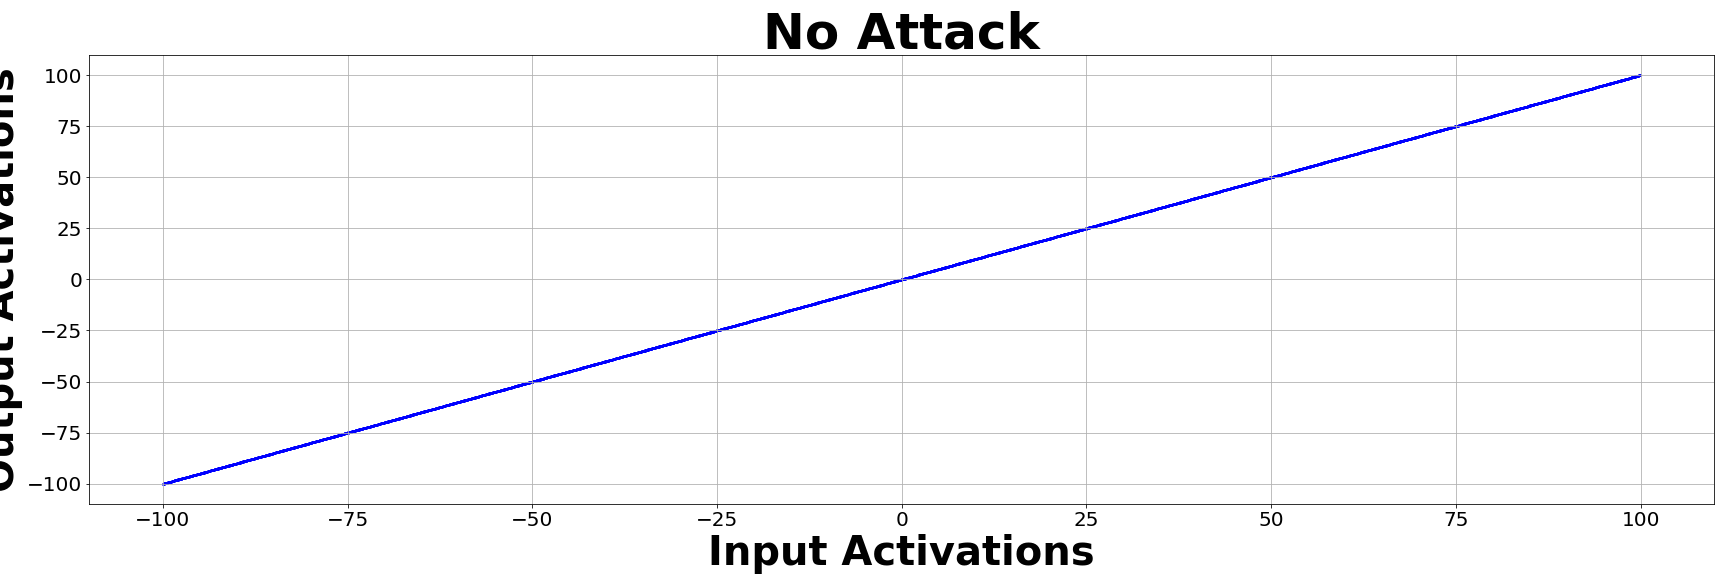
\includegraphics[scale=0.3]{No_Attack}
\end{center}

% ================================================================

\section*{Rounding to the Nearest Integer Value}

\paragraph*{}A simple type of attack model is one that seeks to reduce the numerical accuracy of any values used in floating-point number calculations.  This could be truncating the number, muting bits in the binary representation or simply rounding the values to remove significant figures. For this experiment, we chose to model this type of attack by rounding each floating-point number to the nearest integer value. Thus, in it's base-10 representation, all entries after the decimal point are indentically $0$. We model this attack:

\begin{equation}
\label{round attack}
A_{round} \big[ \hat{W}^{(l)} \vec{x}^{(l)} \big] = \text{ROUND} \big[ \hat{W}^{(l)} \vec{x}^{(l)} ,0 \big]
\end{equation}

Where ROUND[$z,n$] takes from floating-point number $z$ and rounds it to have $n$ decimal places of accuracy in it's base-10 representation; $n$ is an integer. This was functionally done with the package numpy using the function \textit{numpy.round(z,n)}. Visualized:
\begin{center}
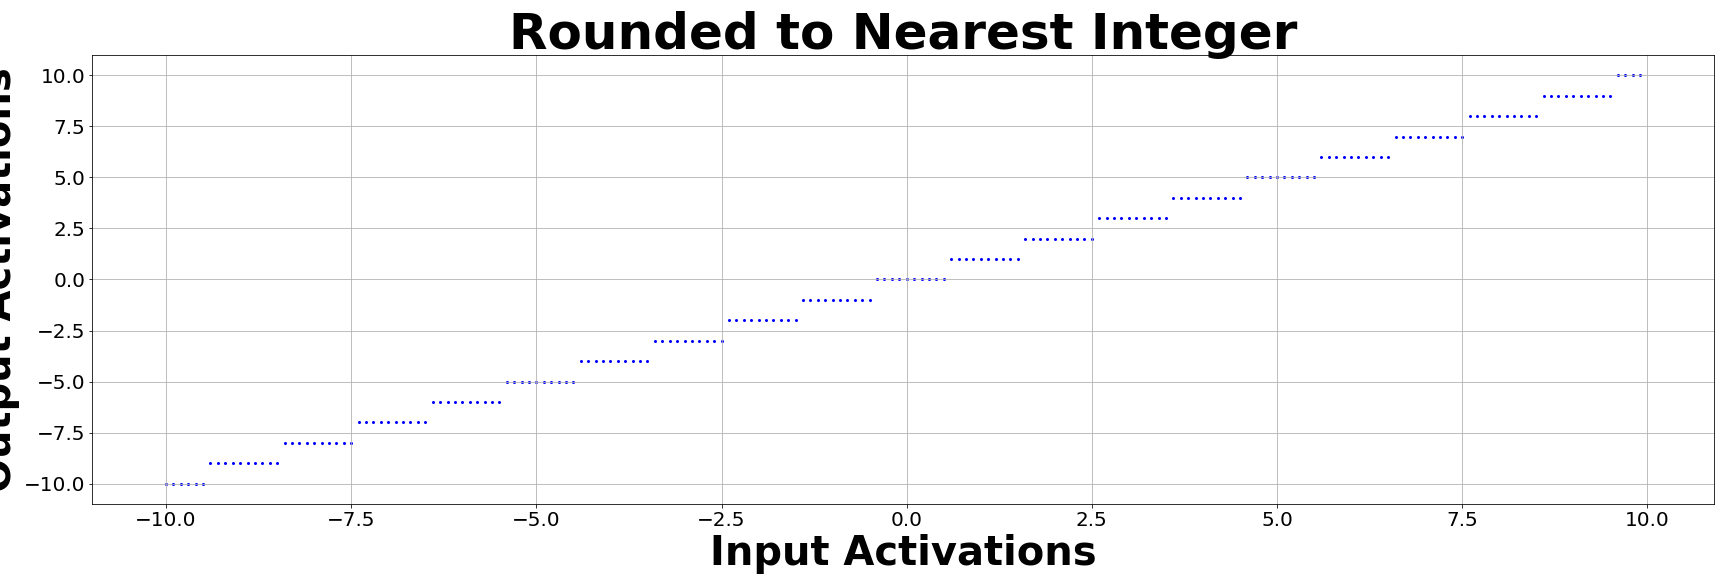
\includegraphics[scale=0.3]{Rounded_to_Nearest_Integer}
\end{center}

% ================================================================

\section*{Adding Noise drawn from a Gaussian Distribution}

\paragraph*{}Another simple type of attack to model is one that introduces inherent noise into the activations of a layer. Mathematically, the attack funtion would take a set of activations, $\vec{x}$ and add noise $\vec{\epsilon}$ as drawn from a distribution or otherwise. Thus we can model an attack function $A$ such that:

\begin{equation}
\label{noise attack}
A_{\text{noise}} \big[ \hat{W}^{(l)} \vec{x}^{(l)} \big] = \hat{W}^{(l)} \vec{x}^{(l)} + \vec{\epsilon}^{(l)}
\end{equation}

To model this numerically, We take the array that results from the matrix-vector product and add an equivalently shaped array containing entries as drawn from a standard Gaussian Distribution, with mean $\mu = 0$ and standard deviation $\sigma = 2$. Thus:
\begin{equation}
\vec{\epsilon}^{(l)} = N(0,2) = \frac{1}{\sqrt{2\pi(2)}} e^{-\frac{x^2}{2(2)}}
\end{equation}
\paragraph*{}To visualize how this affects the activations:
\begin{center}
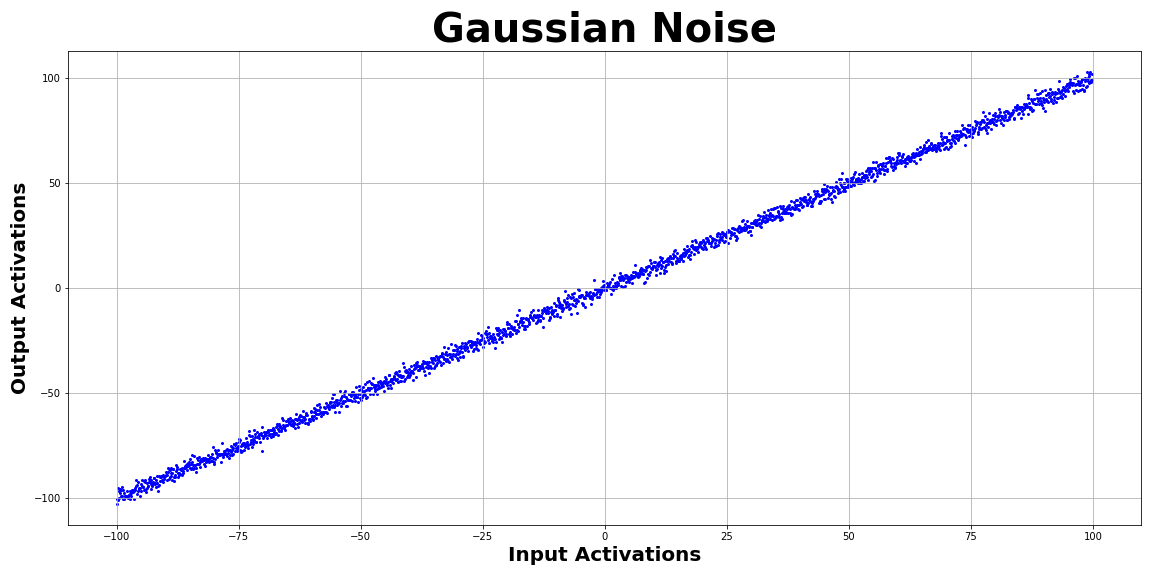
\includegraphics[scale=0.3]{Gaussian_Noise}
\end{center}


% ================================================================

\section*{Muting the Most Significant Bit}

\paragraph*{}In general, when performing computations with Neural Networks, most algorithms with use single or double precision floating point numbers.  In the case of Python 3.7 and Scikit-Learn 0.22.1, these double-precision variant can be set to be used exclusively. To simulate a Network attack at a binary level, we add a filter that 'mutes' the \textit{most-significant-bit} (MSB) in the floating-point number. A Double precision float is composed of 64 binary bits, by the IEEE 754 floating-point standard, the 0-th bit is the sign, the next 11 are the exponent and the remaining 52 are the fraction. Examining just the exponent, we have the 11 bits:

\begin{center}
\begin{tabular}{|c|c|c|c|c|c|c|c|c|c|c|}
\hline
1024 & 512 & 256 & 128 & 64 & 32 & 16 & 8 & 4 & 2 & 1 \\ \hline
- & - & - & - & - & - & - & - & - & - & -  \\ \hline
\end{tabular}
\end{center}

\paragraph*{}Choosing the MSB to be the $1024$ entry, the highest possible value that the exponent can take on is $1023$ (all other bits are 1's). Additionally, with the IEEE 754 standard, there is an exponent offset, that takes the expected exponent value given by the 11 bits and then subtracts $1023$ from it. This means that with the muted first bit and the offset, the exponent part of the float is bounded on the interval 
$e \in [-1023,0]$. We Mathematically show Attack as:

\begin{multline}
\label{mute MSB attack}
A_{\text{MSB}} \big[ \hat{W}^{(l)} \vec{x}^{(l)} \big] = \\
\text{MANT} \big[ \hat{W}^{(l)} \vec{x}^{(l)} \big] \times 2^{E}
\left\{
        \begin{array}{ll}
            E = 0 									&, \text{EXP}[\hat{W}^{(l)} \vec{x}^{(l)}] > 0 \\
            E = EXP[\hat{W}^{(l)} \vec{x}^{(l)}] 	&, \text{otherwise} \\
        \end{array}
    \right.
\end{multline}

Where MANT[$z$] gives the mantissa and EXP[$z$] gives the integer exponent of some floating-point number $z$. In the case of the attack function, $z$ is an element in the objetc resulting from the matrix-vector product.To visualize how this affects the activations:
\begin{center}
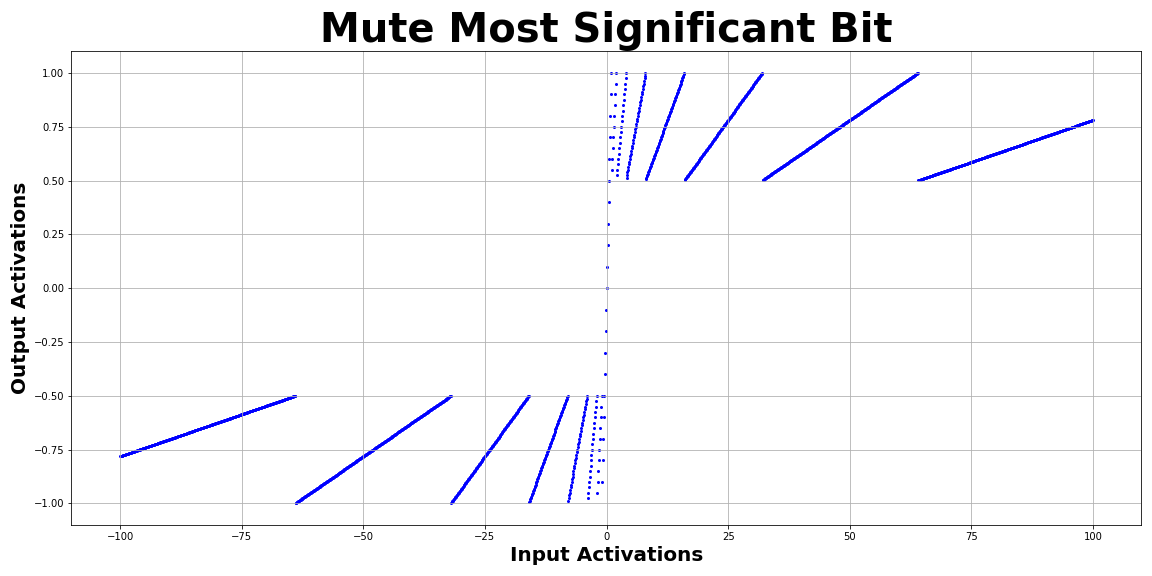
\includegraphics[scale=0.3]{Mute_Most_Significant_Bit}
\end{center}

\paragraph*{}Rather that convert each float to a 64-bit binary string, which is time consuming, we test the value of the exponent in each float using the numpy package function \textit{numpy.frexp(z)}. This operation breaks any floating-point number $z$, into a mantissa $M$ and exponent $E$ such that:
\begin{equation}
z = M * 2^{E}
\end{equation}
If the value of the expoenent $E$, is ever above zero, it is then set to zero and all exponents less than zero are preserved as shown in eqn. (\ref{mute MSB attack}). This has the effect of forcing the double precision float to have an upper bound that asymptotically approaches $2$, but never reach or exceed it.

% ================================================================

\section*{Concluding Remarks}

\paragraph*{}Using three simplified models against a control, we can simulate three different types of possible attacks. In each case, the model is representative of a much larger category of external manipulations. In every case, the attacks targeted the matrix-vector product as shown in eqn. (\ref{attack}) and were triggered by a $50/50$ percent Boolean trigger condition, randomly generated at each forward pass. The Attack functions were set to act on both ther training and testing forward passes, thus constantly affecting a classifiers ability to make a decision, but not it's ability to correct with the Gradient Descent Optimizer.


% ================================================================


\end{document}